\documentclass[border=0.8ex,svgnames,tikz]{standalone}
\usepackage{amsmath,mathtools}
\usepackage{fontspec}
\setmainfont{Source Serif 4}
\setsansfont{Source Sans 3}
\setmonofont{Source Code Pro}

\usetikzlibrary{chains,calc,fit}

\begin{document}
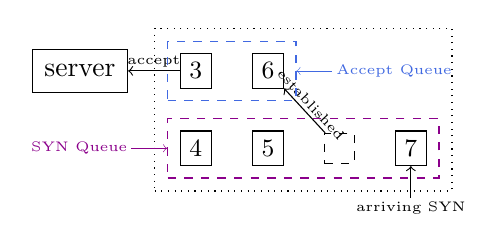
\begin{tikzpicture}
  \begin{scope}[
    every node/.style={
      draw,
      on chain,
      minimum width=8.0ex,
      minimum height=3.6ex,
      font=\normalsize,
    },
    node distance=2em,
    start chain=going below,
    ]
    \node (server) {server};
    \coordinate (tcp);
  \end{scope}
  \coordinate (queue1) at
  ($(server.east)+(server.east)-(server.east)!0.24!(server.center)$);
  \coordinate (queue2) at ($(queue1)+(tcp)-(server)$);
  \begin{scope}[
    every node/.style={
      draw,
      on chain,
      minimum width=2.5ex,
      minimum height=2.5ex,
      font=\small,
    },
    node distance=1.44em,
    start chain=going right,
    ]
    \chainin (queue1);
    \node (queue1-1) {3};
    \node (queue1-2) {6};
    \chainin (queue2);
    \node (queue2-1) {4};
    \node (queue2-2) {5};
    \node[dashed] (queue2-3) {};
    \node (queue2-4) {7};
  \end{scope}
  \begin{scope}[
    fit node/.style n args={3}{fit=#1,inner sep=#2,rectangle,dashed,draw=#3},
    queue node/.style n args={5}{fit node={#1}{#2}{#3},pin={[pin edge={#3,<-}]#4:{\tiny\textcolor{#3}{#5}}}},
    every path/.style={draw,->},
    every node/.style={above,sloped,inner sep=0.3ex,font=\tiny},
    ]
    \path
    (queue1-1) edge node{accept} (server)
    (queue2-3) edge node{established} (queue1-2);
    \path ([yshift=-1.8em]queue2-4) node[below]{arriving SYN} edge (queue2-4);
    \node[fit node={(queue1-1)(queue2-1)(queue2-4)}{9}{Black},dotted]{};
    \node[queue node={(queue1-1)(queue1-2)}{1ex}{RoyalBlue}{right}{Accept
      Queue}]{};
    \node[queue node={(queue2-1)(queue2-4)}{1ex}{DarkMagenta}{left}{SYN Queue}]{};
  \end{scope}
\end{tikzpicture}
\end{document}
